

\chapter{Rabi Oscillations}



\section{Tasks}

\begin{itemize}
\item  Integrate von Neumann eq. / simulations
\end{itemize}



\section{Experiment}

some text


\section{Density Matrix}


We start by introducing the density matrix.\footnote{Rand,  Kap. 3.6 \newline Parson, Kap. 10.2 \newline Hamm 2005, Kap. 1} It is a tool in quantum mechanics to describe not only purely coherent states, but also statistical mixtures, as we will see below. The density matrix is a bit at the edge of the classical canon of quantum mechanics lectures.

When we write our wave function $\ket{\psi}$ in  a basis $\ket{n}$ as
\[
 \ket{\psi} = \sum_n c_n \, \ket{n}
\]
then we can define a density operator $\hat{\rho}$ as
\[
\hat{\rho} =  \ket{\rho}\bra{\rho} = \sum_{m,n} c_n c_m^\star \, \ket{n}\bra{m}
\]
and the matrix elements of $\boldsymbol{\rho}$ are $\rho_{m,n} =  c_n c_m^\star$. The density matrix allows to calculate the expectation value of any operator $\hat{A}$ as
\[
 \braket{\hat{A}} =  \braket{\psi | \hat{A} | \psi}  = \sum_{m,n} c_n c_m^\star \, A_{m,n} = \sum_{m,n} \rho_{n,m} \,  \, A_{m,n} = Tr ( A \rho)
\]
where the trace sums over the diagonal elements
\[
 Tr (U ) = \sum_n U_{n,n} .
\]
The trace of the density matrix is one for normalized states 
\[
 Tr (\rho) = \sum_n \rho_{n,n} = \sum_n c_n c_n^\star = 1 \quad \text{if normalized}
\]
The interesting thing comes when looking at pure and mixed states. Pure states are the 'conventional' states discussed in quantum mechanics, for example this superposition of states
\[
\ket{\psi} = \sqrt{\frac{1}{2}} \left( \ket{1} + \ket{2} \right) 
\]
In this example, the density matrix reads
\[
 \rho = \frac{1}{2} \begin{pmatrix}
 1 & 1 \\ 1 & 1 \\
 \end{pmatrix}
\]
and its trace is one. But the density matrix also allows to describe new things, beyond pure states, namely statistical mixtures of states. We can describe an ensemble of two-level systems, of which half the ensemble is in state $\ket{1}$, the other half in state $\ket{1}$. This can \emph{not} be written as 
$\ket{1} + \ket{2} $, but a density matrix description is possible as
\[
 \rho = \frac{1}{2} \begin{pmatrix}
 1 & 0 \\ 0 & 1 \\
 \end{pmatrix} \quad .
\]
The diagonal elements of the density matrix describe the populations of the states, i.e. $|c_n|^2$. The off-diagonal elements describe coherence between states. In a statistical mixture there is no coherence between the states, as one sub-ensemble is in one state, another in another state. 

We can distinguish between pure and mixed states by looking at the trace of the squared density matrix
\begin{eqnarray*}
 Tr (\rho^2) & = & 1 \quad \text{pure state} \\
 				& < & 1 \quad \text{mixed state} \\
\end{eqnarray*}

Mixed states can be  used not onyl to describe an ensemble of systems in different states, but also to describe a single system that at different times is in different states. Even if we can do an experiment on  a single quantum system, we have to repeat it very often to reduce noise by averaging. But the experiment does not always run along the same path: either a photon is absorbed or not, but it will most likely not always we absorbed. The time-average of such an experiment will thus need  an statistical mixture for its description.

\section{Liouville--von Neumann equation}

We can construct a differential equation for the time evolution of the density matrix that is a direct analogue of the Schrodinger equation, just that is also takes mixed states into account.

The time-derivative of the density matrix $\rho$ is
\[
 \frac{d}{dt} \rho = \frac{d}{dt} \left( \ket{\psi} \bra{\psi} \right) 
 =  \left( \frac{d}{dt}  \ket{\psi} \right) \bra{\psi} 
 + \ket{\psi} \left( \frac{d}{dt}  \bra{\psi} \right) 
\]
Making use of the Schrodinger equation
\[
 \frac{d}{dt} \ket{\psi} = - \frac{i}{\hbar} \, \hat{H} \, \ket{\psi}
\]
we get the Liouville--von Neumann equation
\[
 \frac{d}{dt} \rho = - \frac{i}{\hbar} 
 \left[ \hat{H} , \rho \right]  \quad .
\]

As an example, let us look at a two-level system with the eigen-energies $E_1= 0$ and $E_2 = \hbar \omega_0$. The Hamilton operator is thus
\[
 \hat{H } = \begin{pmatrix}
  0 & 0 \\ 0 & \hbar \omega_0 \\
 \end{pmatrix}
\]
The commutator becomes
\[
 \left[ \hat{H}, \rho \right] = 
 \begin{pmatrix}
 0 & - \hbar \omega_0 \, \rho_{1,2} \\   \hbar \omega_0 \, \rho_{2,1} & 0 \\
 \end{pmatrix}
\]
The  diagonal elements of the density matrix $\rho$, i.e., the populations, remain thus constant in time, as expected for this Hamiltonian. The off-diagonal elements, the coherences acquire a phase-factor proportional to the energy difference, i.e.
\[
 \rho_{1,2}(t) =  \rho_{1,2}(0) \, \exp \left(i \, \omega_0 \, t \right) 
\]

\section{Optical Bloch Equations}

Now we switch on light and add an interaction Hamiltonian $\hat{H}_I = -\boldsymbol{\mu} \, \boldsymbol{E}$ of dipole operator $\boldsymbol{\mu} $ and optical field   $\boldsymbol{E}$. In total, the Hamilton operator reads\footnote{Rand, Kap. 3.8}
\[
 \hat{H } = \begin{pmatrix}
  0 & - {\boldsymbol{\mu}} \, \boldsymbol{E} \\ - {\boldsymbol{\mu}}^\star \, \boldsymbol{E}^\star & \hbar \omega_0 \\
 \end{pmatrix}
\]
The differential equations for the density matrix become the Bloch equations
\begin{eqnarray*}
\dot{\rho}_{00} &=&  - \frac{i}{\hbar} \left( \rho_{10} \boldsymbol{\mu} \, \boldsymbol{E} - \rho_{01} \boldsymbol{\mu}^\star \, \boldsymbol{E}^\star \right) \\
%
\dot{\rho}_{11} &=&  - \frac{i}{\hbar} \left( \rho_{01} \boldsymbol{\mu} \, \boldsymbol{E} - \rho_{10} \boldsymbol{\mu}^\star \, \boldsymbol{E}^\star \right) \\
%
\dot{\rho}_{01} &=& - \frac{i}{\hbar}  \left( - \rho_{01} \hbar \omega_0 + (\rho_{00} - \rho_{11})  \boldsymbol{\mu} \, \boldsymbol{E} \right) \\
%
\dot{\rho}_{10} &=& - \frac{i}{\hbar}  \left( + \rho_{10} \hbar \omega_0 + (\rho_{11} - \rho_{00})  \boldsymbol{\mu}^\star \, \boldsymbol{E}^\star \right) \\
\end{eqnarray*}
We can simplify things by skipping some algebraic transformations and introducing the Bloch vector $\boldsymbol{a}$ with
\[
\boldsymbol{a} = 
\begin{pmatrix}
u \\ v \\ w \\
\end{pmatrix}
= 
\begin{pmatrix}
\rho_{10} + \rho_{01} \\ i (\rho_{10} - \rho_{01}) \\ \rho_{00} - \rho_{11} \\
\end{pmatrix}
= 
\begin{pmatrix}
\Re (\rho_{10})  \\ \Im (\rho_{10}) \\ \rho_{00} - \rho_{11} \\
\end{pmatrix}
\]
With this we can write the system of differential equation as 
\[
 \dot{\boldsymbol{a}} = \boldsymbol{M}   \times \boldsymbol{a} 
 \quad \text{with} \quad 
 \boldsymbol{M}  = 
 \begin{pmatrix}
 \frac{2}{\hbar} \, \Re ( \boldsymbol{\mu} \, \boldsymbol{E} ) \\
  \frac{2}{\hbar} \, \Im ( \boldsymbol{\mu} \, \boldsymbol{E} ) \\
  \omega_0
 \end{pmatrix}
\]
The time evolution of the density matrix, of the Bloch vector, can be described by the action of a torque vector $\boldsymbol{M}$ on the Bloch vector. Without optical field, the Bloch vector rotates around its $w$ axis, as seen in the phase oscillation of the coherences in the last chapter. With optical field, also the populations changes, and things become complicated.

To simplify things, we assume that our optical field is a single mode with a slowly varying amplitude only, i.e.
\[
 \boldsymbol{E}(t) = \boldsymbol{x} \, E_0(t) \left( e^{i \omega_L t} + e^{-i \omega_L t} \right)
\]
The time-dependence of $E(t)$ should be slow compared to $\omega_L t$. This is the slowly-varying amplitude approximation (SVEA). Then we move into a rotating frame. Our new coordinate system rotates around the $w$ axis with the angular frequency of the laser $\omega_L$. The optical frequency of the transition $\omega_0$ is close to this laser frequency. We neglect terms of $\omega_0 + \omega_L$ and only keep terms of  $\omega_0 - \omega_L$. The first will oscillate fast and average out, the latter oscillate slowly. This is the rotating wave approximation (RWA). In total we get in the rotating frame 
\[
 \dot{\boldsymbol{a}'} = \boldsymbol{M}'   \times \boldsymbol{a}' 
 \quad \text{with} \quad 
 \boldsymbol{M}'  = 
 \begin{pmatrix}
2 \boldsymbol{\mu}  \boldsymbol{x}   |E(t)| / \hbar \\
0 \\
\omega_0 - \omega_L
 \end{pmatrix} = 
  \begin{pmatrix}
\Omega \\
0 \\
\omega_0 - \omega_L
 \end{pmatrix}
\]
with the (angular) Rabi frequency $\hbar \Omega = 2 \boldsymbol{\mu}  \boldsymbol{x}   |E(t)| $.






\section{9.1. Rabi-Oszillationen\protect\footnote{Rand, Kap. 4.1, Simon Biberger}\hfill ***} 

\textit{Das Zwei-Niveau-System oszilliert entweder als Funktion der
Zeit oder der 'pulse area' zwischen Grund- und angeregtem
Zustand.}\\
Betrachtet man ein Atom, das plötzlich Licht ausgesetzt ist, welches resonant mit einem Übergang aus dem Grundzustand ist. So kann es zu einem kohärenten transienten Phänomen kommen, der Nutation. Die Nutation beschreibt den Aufbau einer Polarisation, welche durch die Anwesenheit eines optischen Feldes verursacht wird.\\
Da die Rabi-Oszillationen in Bezug auf Populationszerfälle schnelle Prozesse sind, vereinfachen sich die Bloch-Gleichungen zu:
\begin{align}
    \dot{R_1} =& -\Delta R_2  \notag \\
    \dot{R_2} =& \Delta R_1 + \Omega R_3 \label{Rabi}\\
    \dot{R_3} =& - \Omega R_2 \notag
 \end{align}
Diese Gleichungen lassen sich bei Mitnahme eines möglichen Doppler-Shifts ($v_z$) und mit einer Anfangsverteilung der Population $R_3$(0) lösen.
\begin{align}
    R_1(t) =& \frac{\Omega \Delta}{\Omega_R^2}R_3(0)\cdot cos(\Omega_Rt-1) \notag \\
    R_2(t) =& \frac{\Omega}{\Omega_R}R_3(0)\cdot sin(\Omega_Rt) \label{Rabi2}\\
    R_3(t) =& R_3(0)\cdot \left[1+\frac{\Omega^2}{\Omega_R^2}\cdot 
    cos(\Omega_Rt-1)\right] \notag
\end{align}
Dabei ist $\Omega_R^2$ = $\Delta^2 + \Omega^2$, $\Delta = \omega_0-\omega-kv_z$ und $\Omega = \mu_{21}E_{12}/\hbar$.\\
Der Betrag des Bloch-Vektors bleibt über die betrachtete Zeit konstant. Er präzediert um den Vektor $\bar{\beta}$ mit der Frequenz $\Omega_R$.
Für den Resonanzfall $\Delta = 0$ kommt es zum Rabi-flopping. Dabei springt  $\bar{\beta} = \Omega \hat{e}_1$ auf $\bar{\beta} = -\Omega \hat{e}_1$. Das Atom oszilliert also zwischen dem angeregten und Grundzustand unter dem Einfluss eines treibenden Feldes.\\
Die Rabi-Oszillationen können über zwei Methoden gemessen werden. Entweder betrachtet man die Zeitentwicklung der Fluoreszenz bei einem festen treibenden Feld oder die Transmissionsänderung während der Variation der treibenden Feldes.
\begin{figure} [h]
    \centering
    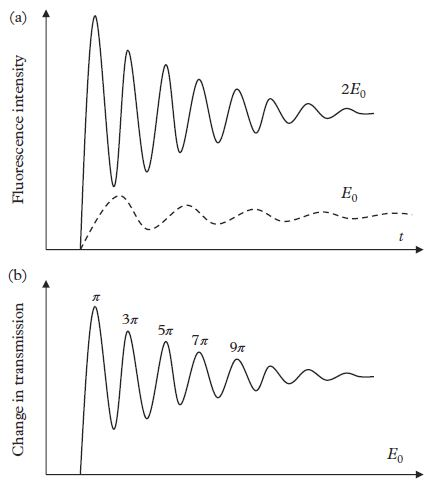
\includegraphics[width = 0.7 \textwidth]{\currfiledir/Rabi1.JPG}
    \caption{Rabi-Oszillationen in (a) transienter Fluoreszenz und (b) differentielle Transmissionsmessung.}
    \label{fig:Rabi}
\end{figure}


\section{RESTE}

Um den Hermiteschen Charakter des Hamilton-Operators zu erhalten, muss beim Beachten von Zerfallstermen die Bewegungsgleichung folgendermaßen modifiziert werden.
\begin{align}
    i\hbar \dot{\hat{\rho}} =& [\hat{H},\hat{\rho}] + Relaxationsterme \notag\\
    =& [\hat{H},\hat{\rho}] \pm i\hbar\Lambda \pm i\hbar\gamma \hat{\rho} - i\hbar \Gamma \hat{\rho}
\end{align}


Der erste Term berücksichtigt die Abnahme durch inkohärentes Pumpen, der zweite die strahlende und nicht-strahlende Populations-Relaxation. Der letzte beachtet das dephasing. 


Polarization und abgestrahlte Felder\protect\footnote{Rand, Kap. 3.9}
Wie kommt es, dass man am Ende etwas detektieren kann? 


\printbibliography[segment=\therefsegment,heading=subbibliography]
